\renewcommand\thefigure{\thesection.\arabic{figure}} % To caption images properly for appendix
\renewcommand\thetable{\thesection.\arabic{table}} % To caption images properly for appendix
\setcounter{figure}{0}
\setcounter{table}{0}

\subsection{Standards} \label{app:standards}

\begin{center}
    \begin{longtable}{ | p{2.2cm} | p{2.5cm} | p{4cm} |p{6cm}|}
        \caption{List of possible Standards and Regulations}
        \label{table:standards}
        \\ \hline
        Organization & Standard Number & Standard Name & Description
        \\ \hline
        ASTM & E2991 / E2991M - 17 & Evaluating Response Robot Mobility: Traverse Gravel Terrain. & Test method to determine capability of robot in gravel terrain \cite{astm_standard_nodate}.
         \\ \hline
        ASTM & E2992 / E2992M - 17 & Evaluating Response Robot Mobility: Traverse Sand Terrain. & Test method to determine capability of robot in sand terrain \cite{astm_standard_nodate-1}.
        \\ \hline
        ISO & 15066:2016 & Robots and robotic devices & Specifies collaborative robot safety requirements \cite{iso_iso/ts_nodate}.
        \\ \hline
        ISO & 10218-1:2011 & Safety Requirements for industrial robots. Part 1: Robots & Specifies requirements and guidelines for the inherent safe design, protective measures and information for use of industrial robots \cite{iso_iso_nodate-1}.
        \\ \hline
        ISO & 13482:2014 & Safety requirements for personal care robots & Provides requirements to eliminate, or reduce, the risks associated with these hazards \cite{iso_iso_nodate}.
        \\ \hline
        ISO & 18646-2:2019 & Performance criteria and related test methods for service robots -- Part 2: Navigation & Test method to determine mobility service of robot \cite{iso_iso_nodate-2}.
        \\ \hline
        ISO & 13849-1:2015 & Safety-related parts of control systems -- Part 1: General principles for design & Safety requirements for the design and integration of safety related parts \cite{iso_iso_nodate-3}.
        \\ \hline
        ISO & 13850:2015 & Emergency stop function & Requirement and principle for the design of emergency stop function \cite{iso_iso_nodate-4}.
        \\ \hline
        ISO & 13854:2017 & Minimum gaps to avoid crushing of parts of the human body & Avoiding hazards in crushing zones \cite{iso_iso_nodate-8}.
        \\ \hline
        ISO & 13855:2010 & Positioning of safeguards with respect to the approach speeds of parts of the human body & Parameter specification for approach speed of parts of the human body \cite{iso_iso_nodate-5}.
        \\ \hline
        ISO & 14118:2017 & Prevention of unexpected start-up & Requirements in the design to prevent unexpected machine start up \cite{iso_iso_nodate-6}.
        \\ \hline
        ISO & 13857:2008 & Safety distances to prevent hazard zones being reached by upper and lower limbs & Establishes safety distances from hazard zones \cite{iso_iso_nodate-7}.
        \\ \hline
        RIA & R15.06-2012 &  Industrial Robots and Robot Systems- Safety Requirements & Safety requirements for the design and use of \cite{ansi_ansi/ria_nodate}.
        \\ \hline
        RIA & TR15.606-2016 & Collaborative Robots & Safety requirements specific to collaborative robots \cite{ria_ria_nodate}.
        \\ \hline
        Canada & N/A & Hazardous Products Act & Compliance to all regulations set by Health Canada \cite{canada_hazardous_2019}.
        \\ \hline
        Canada & N/A & Consumer Product Safety Act & Compliance set by Health Canada \cite{canada_canada_2011}
         \\ \hline
        IEC & 60529 & Ingress Protection Marking & Capacity of an electronic device to protect against the intrusion of solid objects, dust and water \cite{dstm_ip_nodate}.
        \\ \hline
       
    \end{longtable}
\end{center}


\subsection{MiniHyQ} \label{app:minihyq}

Linear hydraulic actuators are no longer available from Fluitronics; the spec sheet for the Hydro-Lek HLK 14000 is below.
This is an alternative actuator provided by Khan in his analysis \cite{khan_development_2015} with similar operating pressure and dimensions.

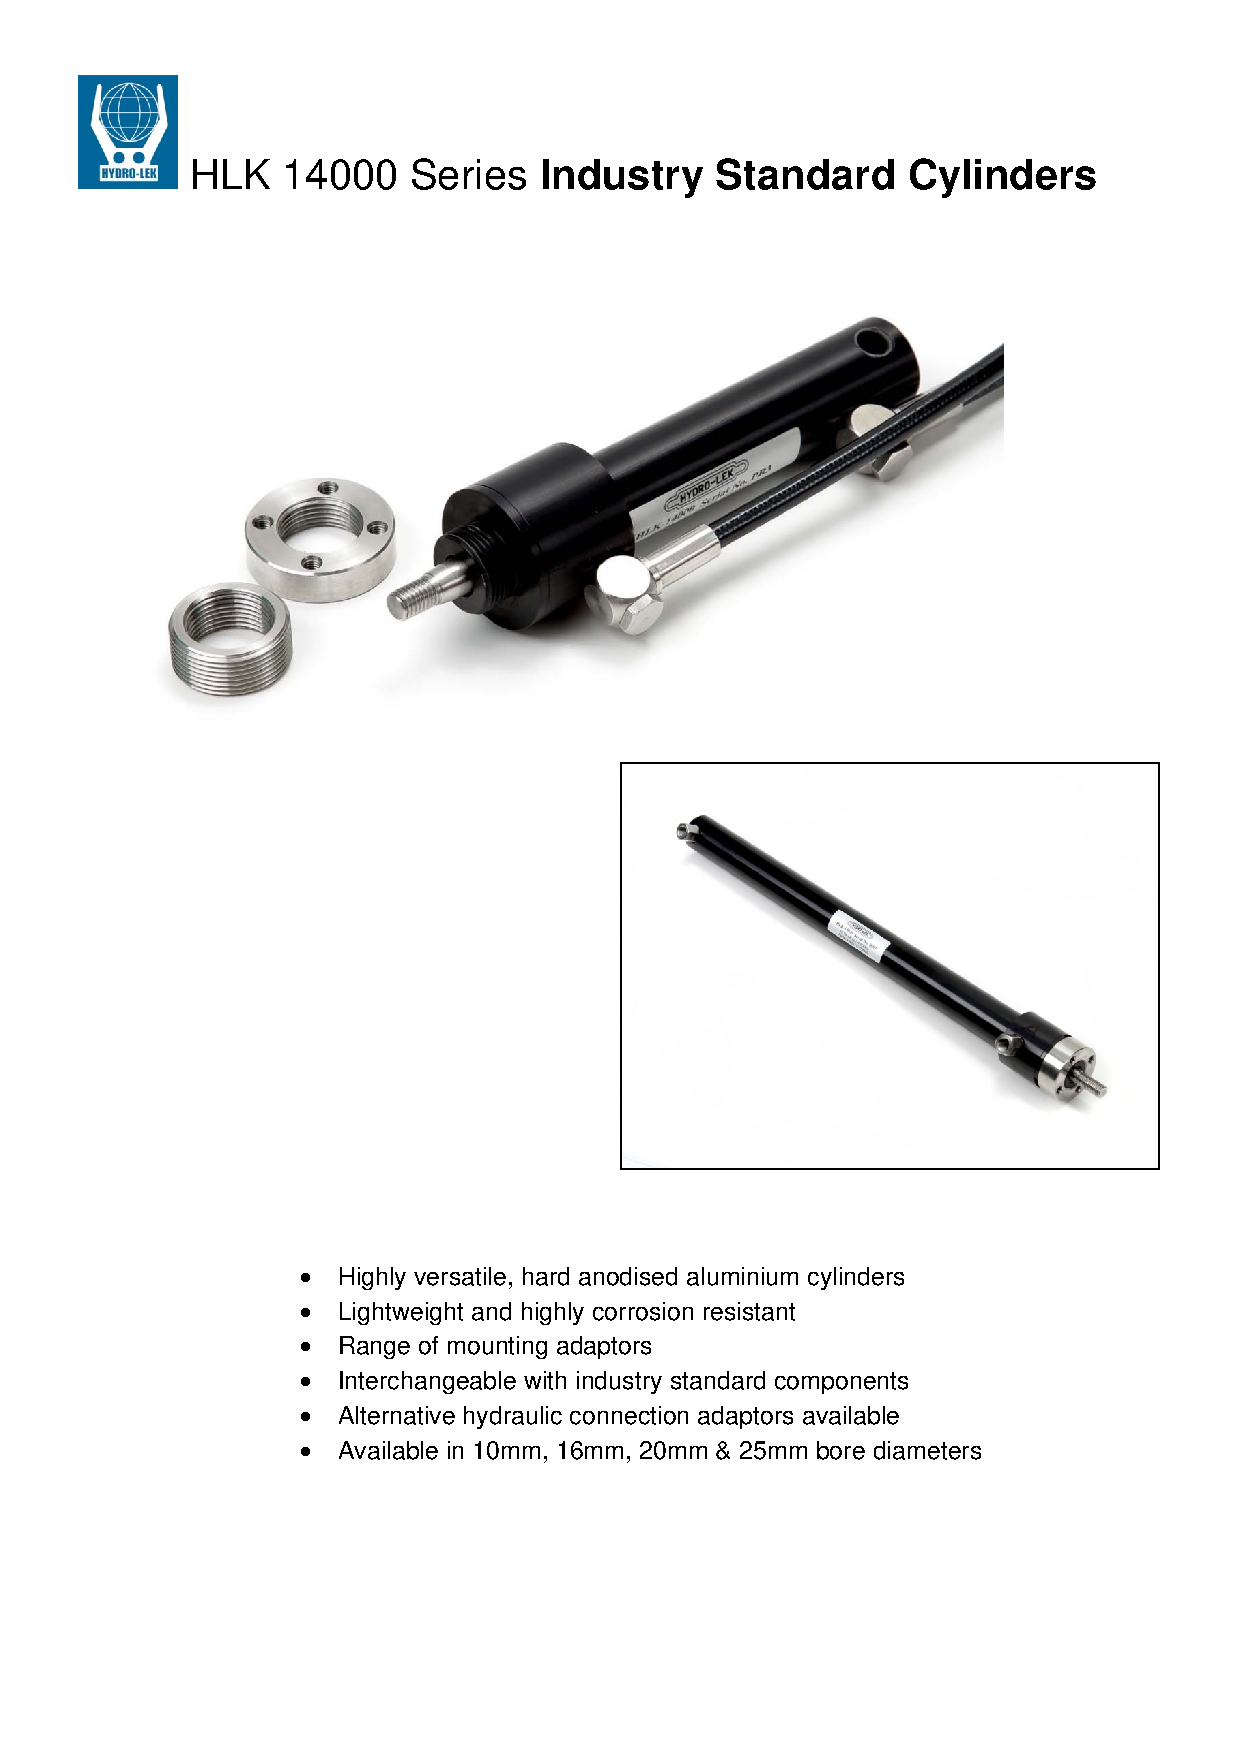
\includepdf[pages=-]{hydrolek-HLK14000.pdf}


\subsection{Custom Gasket Materials from Protocase Manufacturer} \label{app:gaskets}

As an example of possible gasket materials and applications, the available materials from Protocase are shown below \cite{protocase_custom_nodate}.

\begin{figure}[H]
    \centering
    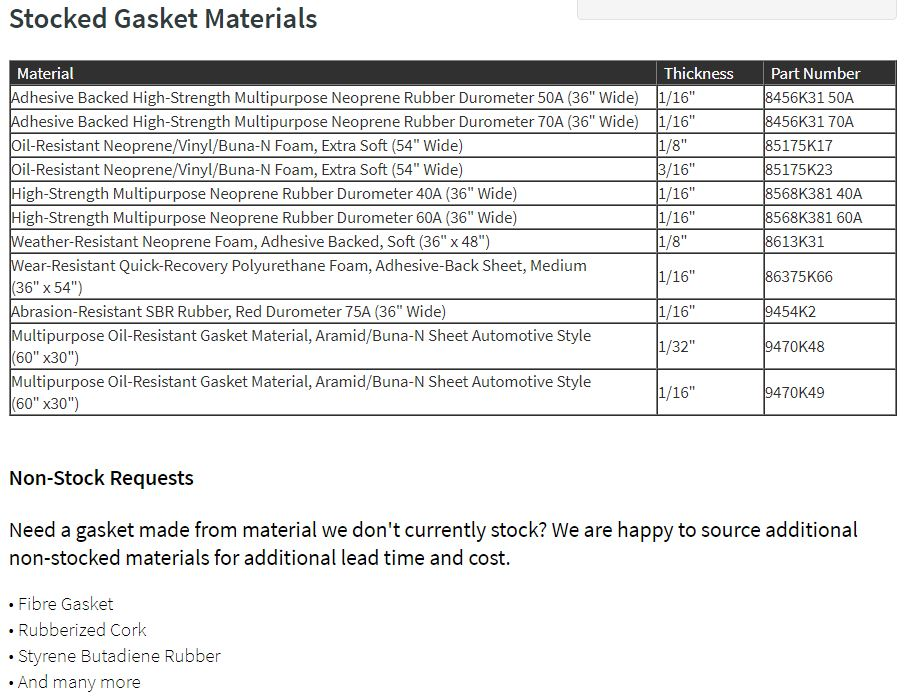
\includegraphics[width=0.9\textwidth]{Sections/Appendices/Appendix_Gasket.JPG}
    \caption{Custom gasket materials from Protocase \cite{protocase_custom_nodate}}
    \label{fig:appendix_gasket}
\end{figure}

\subsection{Angular Contact Bearings Arrangement} \label{app:bearings}

Based on the magnitude and direction of the radial and thrust loads, multiple arrangements combining sets of bearings are possible and presented in Figure \ref{fig:bearing_arrang}.

\begin{figure}[H]
    \centering
    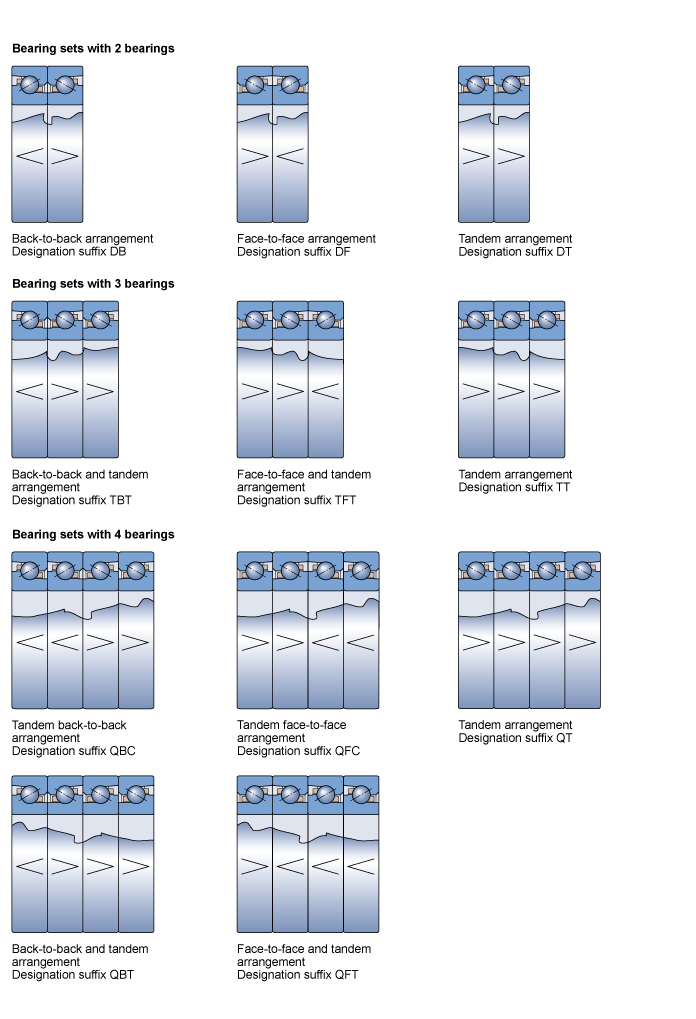
\includegraphics[width=0.9\textwidth]{Sections/Appendices/bearings_arrang.png}
    \caption{Multiple examples of back-to-back, face-to-face, and tandem arrangements for different sets of angular contact ball bearings \cite{skf_bearing_nodate}}
    \label{fig:bearing_arrang}
\end{figure}


\subsection{Materials and Coatings} \label{app:materials}

As an outdoor application, corrosion free and weather proof materials are required. Aluminum, Stainless Steels, Galvanized Steel and Red Metals (Copper, Brass and Bronze)\cite{media_metals_2018}\cite{form_best_nodate}\cite{noauthor_4_2018}.

As \textbf{Aluminum} contain almost no iron in its composition, it cannot rust. In addition, when exposed to water, the aluminum will create an aluminum oxide layer creating an additional rust barrier and protecting the metal underneath. Aluminum is found in aircraft, cars and bicycles. Aluminum will corrode easily when exposed to salt \cite{media_metals_2018}\cite{form_best_nodate}\cite{noauthor_4_2018}.

\textbf{Galvanized steel} is also durable against rust. It is the zinc protective coat on the steel that protects the steel from rusting. In extreme environments, the zinc layer will be rendered ineffective in such causing the steel to rust. Water and condensation can oxidize the zinc coating, called white rust. Galvanized steel is specially used do to its affordable price \cite{media_metals_2018}\cite{form_best_nodate}\cite{noauthor_4_2018}.

Other metals containing almost no iron and are considered highly durable and resistant are the Red Metals, which includes \textbf{Copper, Bronze and Brass}. However, red metals do oxide forming a green layer protecting the metal from further oxidation \cite{media_metals_2018}\cite{form_best_nodate}\cite{noauthor_4_2018}.

Stainless steel is another great outdoor weather proof material due to its durability and inability to rust. The most common grades for outside use includes 304 and 316 due to its high composition of nickel and chromium \cite{media_metals_2018}\cite{form_best_nodate}\cite{noauthor_4_2018}.

Plastics can also be great materials for outdoor use. The best plastics for outdoor use includes Acrylic, Polycarbonate, HDPE \cite{noauthor_uv_nodate}\cite{marla_acme_best_2019}. 

\textbf{Acrylic} has high weather resistance, work in temperature ranging from -40 to 180 degree Fahrenheit, and is UV stabilized \cite{noauthor_uv_nodate}\cite{marla_acme_best_2019}.

Another UV stabilized plastic is \textbf{Polycarbonate}, with work temperature from -40 to 240 degree Fahrenheit and excellent with high impact resistance \cite{noauthor_uv_nodate}\cite{marla_acme_best_2019}.

\textbf{Polyethylene HDPE} has high abrasion and corrosion resistance properties with a reasonable impact strength and operates under 32 to 210 degrees Fahrenheit.However, the plastic is not UV stabilized and less resistant to sun rays \cite{noauthor_uv_nodate}\cite{marla_acme_best_2019}.  

As an alternative to waterproof and corrosion resistant material for the design which can have additional cost over other cheaper steels and metals, rust coating and anti corrosion coating can provide waterproof and chemical proof properties, protect against organism such fungi, algae and moss, and resist harsh environments including acid rain and salt water.

To properly coat a metal, multiple layers of coating must be applied. In order of operations: Primer, Sealer, Intermediate Coat, and Finishing Coat. All layers and specifically the intermediate coat will also depend on the degree of corrosivity exposed to the metal \cite{noauthor_anti_nodate}.

\begin{figure}[H]
    \centering
    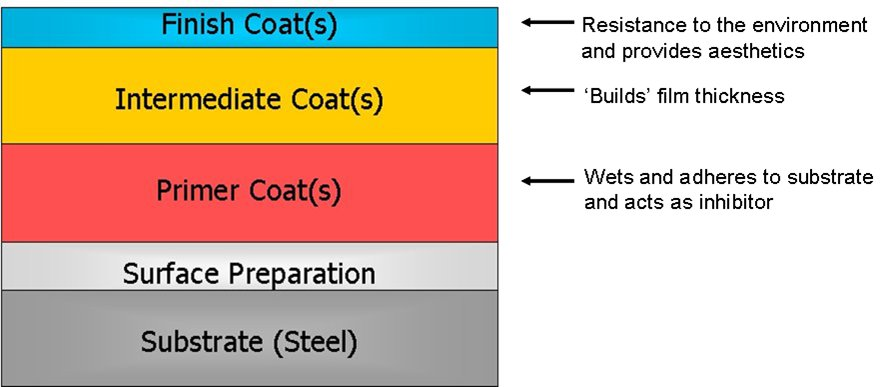
\includegraphics[width=0.5\textwidth]{Sections/LiteratureReview/img/coat_paint.jpg}
    \caption{Typical paint system diagram \cite{noauthor_paint_nodate}}
    \label{fig:paint}
\end{figure}


\subsection{Physical Seal of Enclosure Using Welding} \label{app:sealing}

It is possible to weld the chassis to provide a physical seal against the elements. This option is a permanent seal, thus the previous solutions shown in the static seals section may still be needed for easily-removable maintenance points. One potential process is seam welding which consists of passing two overlapped sheet metal parts between two wheel-shaped electrodes. The current then goes through the parts, and their contact resistance causes them to heat up and coalesce together, as shown in figure \ref{fig:welding_RSEW}. This method is useful to weld seams in conductive materials, and is efficient at creating waterproof seals \cite{weman_welding_2012}. 

\begin{figure}[H]
    \centering
    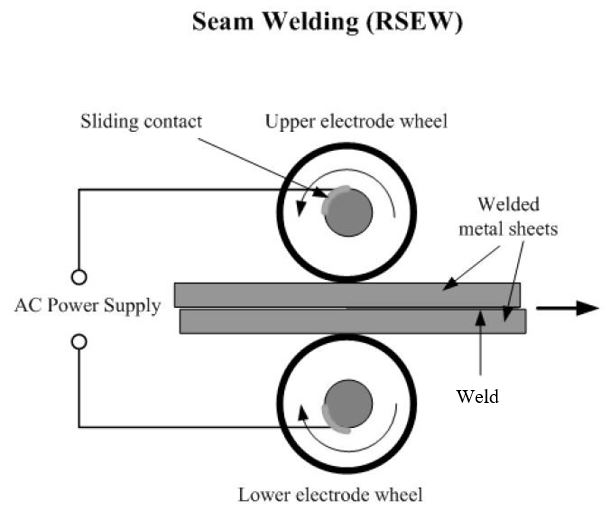
\includegraphics[width=0.6\textwidth]{Sections/LiteratureReview/img/seals/welding_RSEW.JPG}
    \caption{Resistance Seam Welding Method \cite{alawi_modal_2017}}
    \label{fig:welding_RSEW}
\end{figure}

Another process, which can be used with plastics, is ultrasonic welding. This process uses high frequency vibrations and pressure to create a weld,as shown in figure \ref{fig:welding_USW}. This process is often used in the packaging industry and can thus provide a leak-proof weld. It is also used with a wide variety of materials \cite{weman_welding_2012} \cite{telsonic_plastic_nodate}.

\begin{figure}[H]
    \centering
    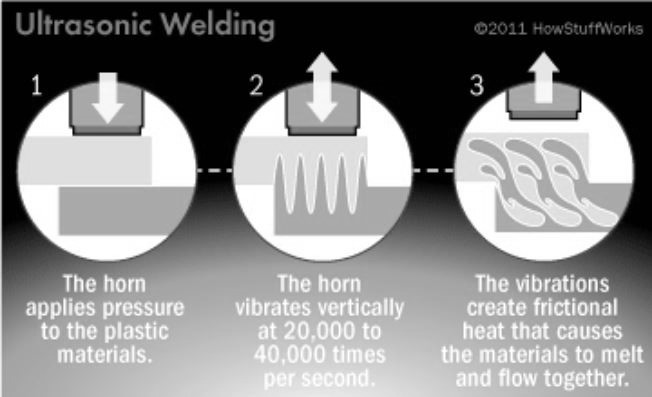
\includegraphics[width=0.5\textwidth]{Sections/LiteratureReview/img/seals/welding_USW.JPG}
    \caption{Ultrasonic Welding Method \cite{freudenrich_how_2011}}
    \label{fig:welding_USW}
\end{figure}


\subsection{Interior Dynamic Seals} \label{app:dynamicseals}

Rotary shaft lip seals are available in many shapes and materials for different applications. Figure \ref{fig:seal_rotary2} shows the mounting of a lip seal that is oriented to exclude contaminants from a bearing \cite{skf_external_nodate}. These seals generally have a metal shell that is press mounted to fit in a bore in the housing \cite{skf_seal_nodate}. 

\begin{figure}[H]
    \centering
    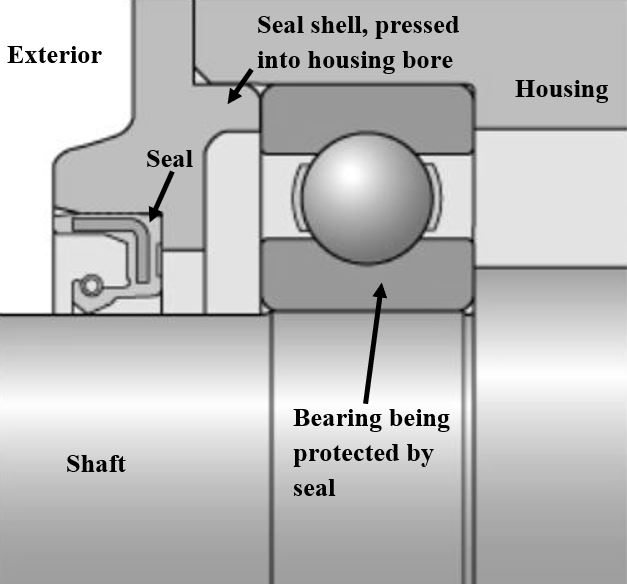
\includegraphics[width=0.5\textwidth]{Sections/LiteratureReview/img/seals/seal_rotary2.JPG}
    \caption{Possible configuration and mounting of a rotary lip seal \cite{skf_external_nodate}}
    \label{fig:seal_rotary2}
\end{figure}

Similar seals, called U-Cup seals, are available for reciprocating motion applications (see figure \ref{fig:seal_linear2}). For mounting, they are generally compressed within a groove in the housing or shaft/piston. Both these types of seals are useful to keep most particles, such as sand and dirt, out of a system, but are often meant to use in lightweight applications and may not be completely waterproof \cite{shigley_standard_2004}. 

\begin{figure}[H]
    \centering
    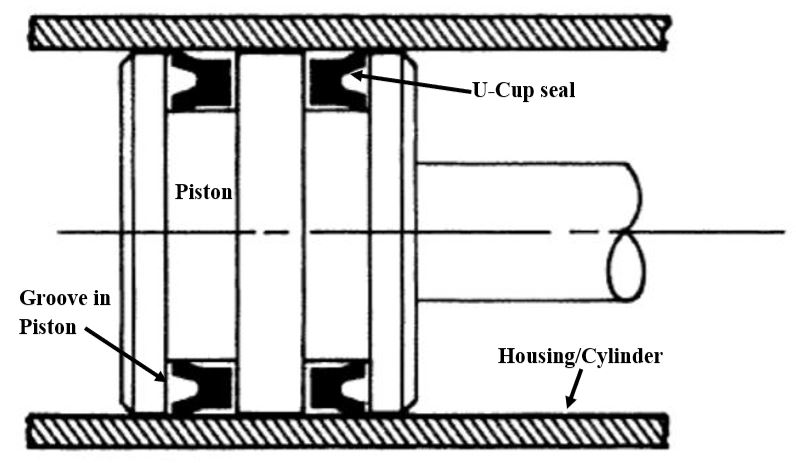
\includegraphics[width=0.6\textwidth]{Sections/LiteratureReview/img/seals/seal_linear2.JPG}
    \caption{U-Cup seals used on a piston \cite{shigley_standard_2004}}
    \label{fig:seal_linear2}
\end{figure}

To provide a waterproof seal on a rotating shaft, a mechanical seal can be used. Although they may have different configurations, they usually function by having two rings: one rotating with the shaft and the other stationary and fixed to the housing. The seal is thus provided at the shaft, at the housing and between the two rings which are in contact \cite{ali_m._sadegh_marks_2018} \cite{green_perrys_2019}. An example of the mounting of a mechanical seal is shown in figure \ref{fig:mechseal}. 

\begin{figure}[H]
    \centering
    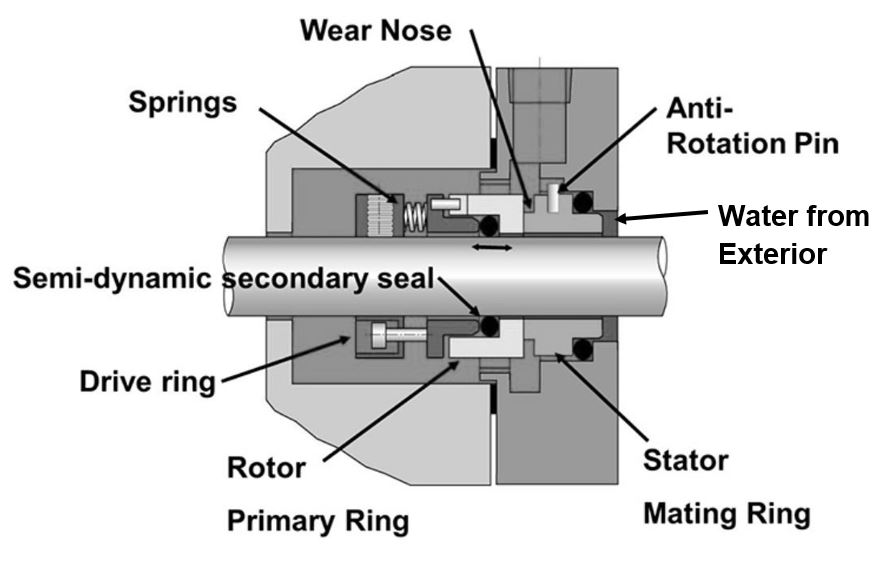
\includegraphics[width=0.6\textwidth]{Sections/LiteratureReview/img/seals/mechseal.JPG}
    \caption{Possible configuration and mounting of a mechanical seal \cite{attenasio_back_2016}}
    \label{fig:mechseal}
\end{figure}

\subsection{Hydraulic} \label{app:hydraulic}

For MiniHyQ, Moog E024 servo valves were selected for actuation control, while a TAKAKO axial piston pump, Neu motor 10kW DC motor and single stage 6.5:1 planetary gearbox manage the hydraulic circuit \cite{khan_development_2015-1}.

\begin{figure}[H]
    \centering
    \includegraphics[width=0.7\textwidth]{Sections/LiteratureReview/img/minihyq/subsys_minihyq_moog.png}
    \caption{Moog servo valve assembly for front or rear legs \cite{khan_development_2015-1}}
    \label{fig:minihyq_hydraulic_moog}
\end{figure}

\begin{figure}[H]
    \centering
    \includegraphics[width=0.7\textwidth]{Sections/LiteratureReview/img/minihyq/subsys_minihyq_pump.png}
    \caption{MiniHyQ hydraulic Neu motor and TAKAKO pump \cite{khan_development_2015-1}}
    \label{fig:minihyq_hydraulic_pump}
\end{figure}

Figure \ref{fig:hydraulic_linear_system} and Figure \ref{fig:hydraulic_linear_schematic} demonstrate typical components of a hydraulic system for an actuator; in both cases the actuator is linear, however the linear actuator can be replace by rotary actuator and other types of hydraulic actuator. 

Typical hydraulic system includes the following component: hydraulic pump paired with a motor, directional control valve to control the pressure and the flow of the liquid (water), filter, and a reservoir for the excess liquid in the system. Pressure gauge are installed across the system to monitor the pressure in the system but are not essential to the functionality of the system, the pressure relief valve enables to control the pressure in the system by enabling the liquid to discharge from the valve when high pressure levels are reached.

\begin{figure}[H]
    \centering
    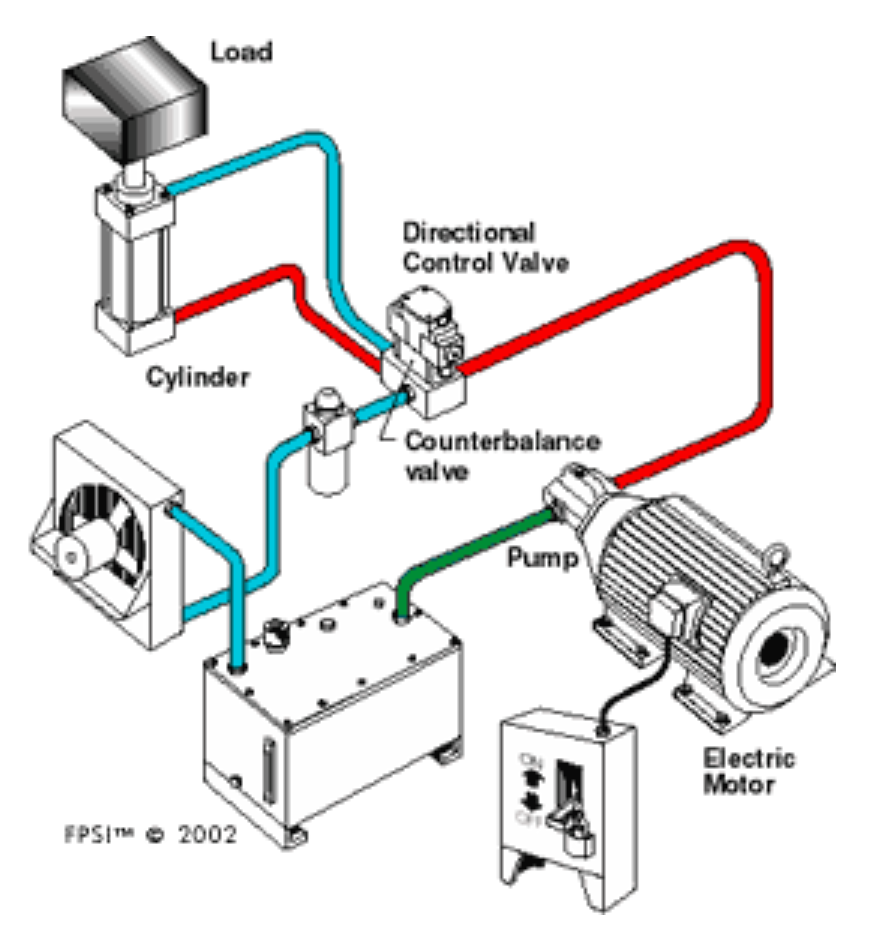
\includegraphics[width=0.5\textwidth]{Sections/LiteratureReview/img/drive/Hydraulic_linear_actuator.png}
    \caption{Basic hydraulic system for linear activator \cite{fluid_power_safety_fluid_nodate}}
    \label{fig:hydraulic_linear_system}
\end{figure}

\begin{figure}[H]
    \centering
    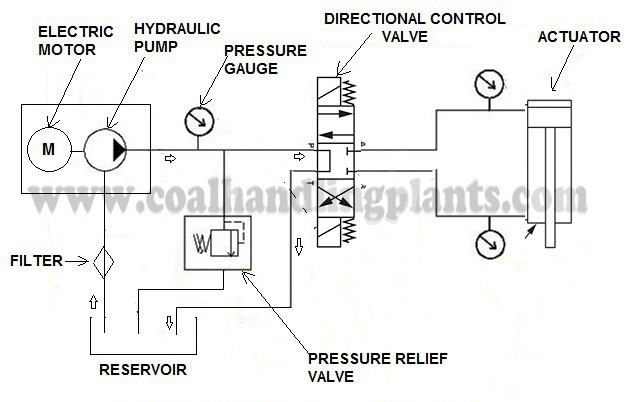
\includegraphics[width=0.5\textwidth]{Sections/LiteratureReview/img/drive/hydraulic_schematic.jpg}
    \caption{Basic hydraulic system for linear activator schematic \cite{coal_handling_plants_basic_2017}}
    \label{fig:hydraulic_linear_schematic}
\end{figure}

\subsection{Solar Panel Specifications from Wholesale Solar} \label{app:solar}

The following are the specifications from Wholesale Solar for a 100 W rigid solar panel recommended for RV's \cite{wholesale_solar_solarland_nodate} and a 100W flexible solar panel recommended for RV's \cite{wholesale_solar_sunpower_nodate}.

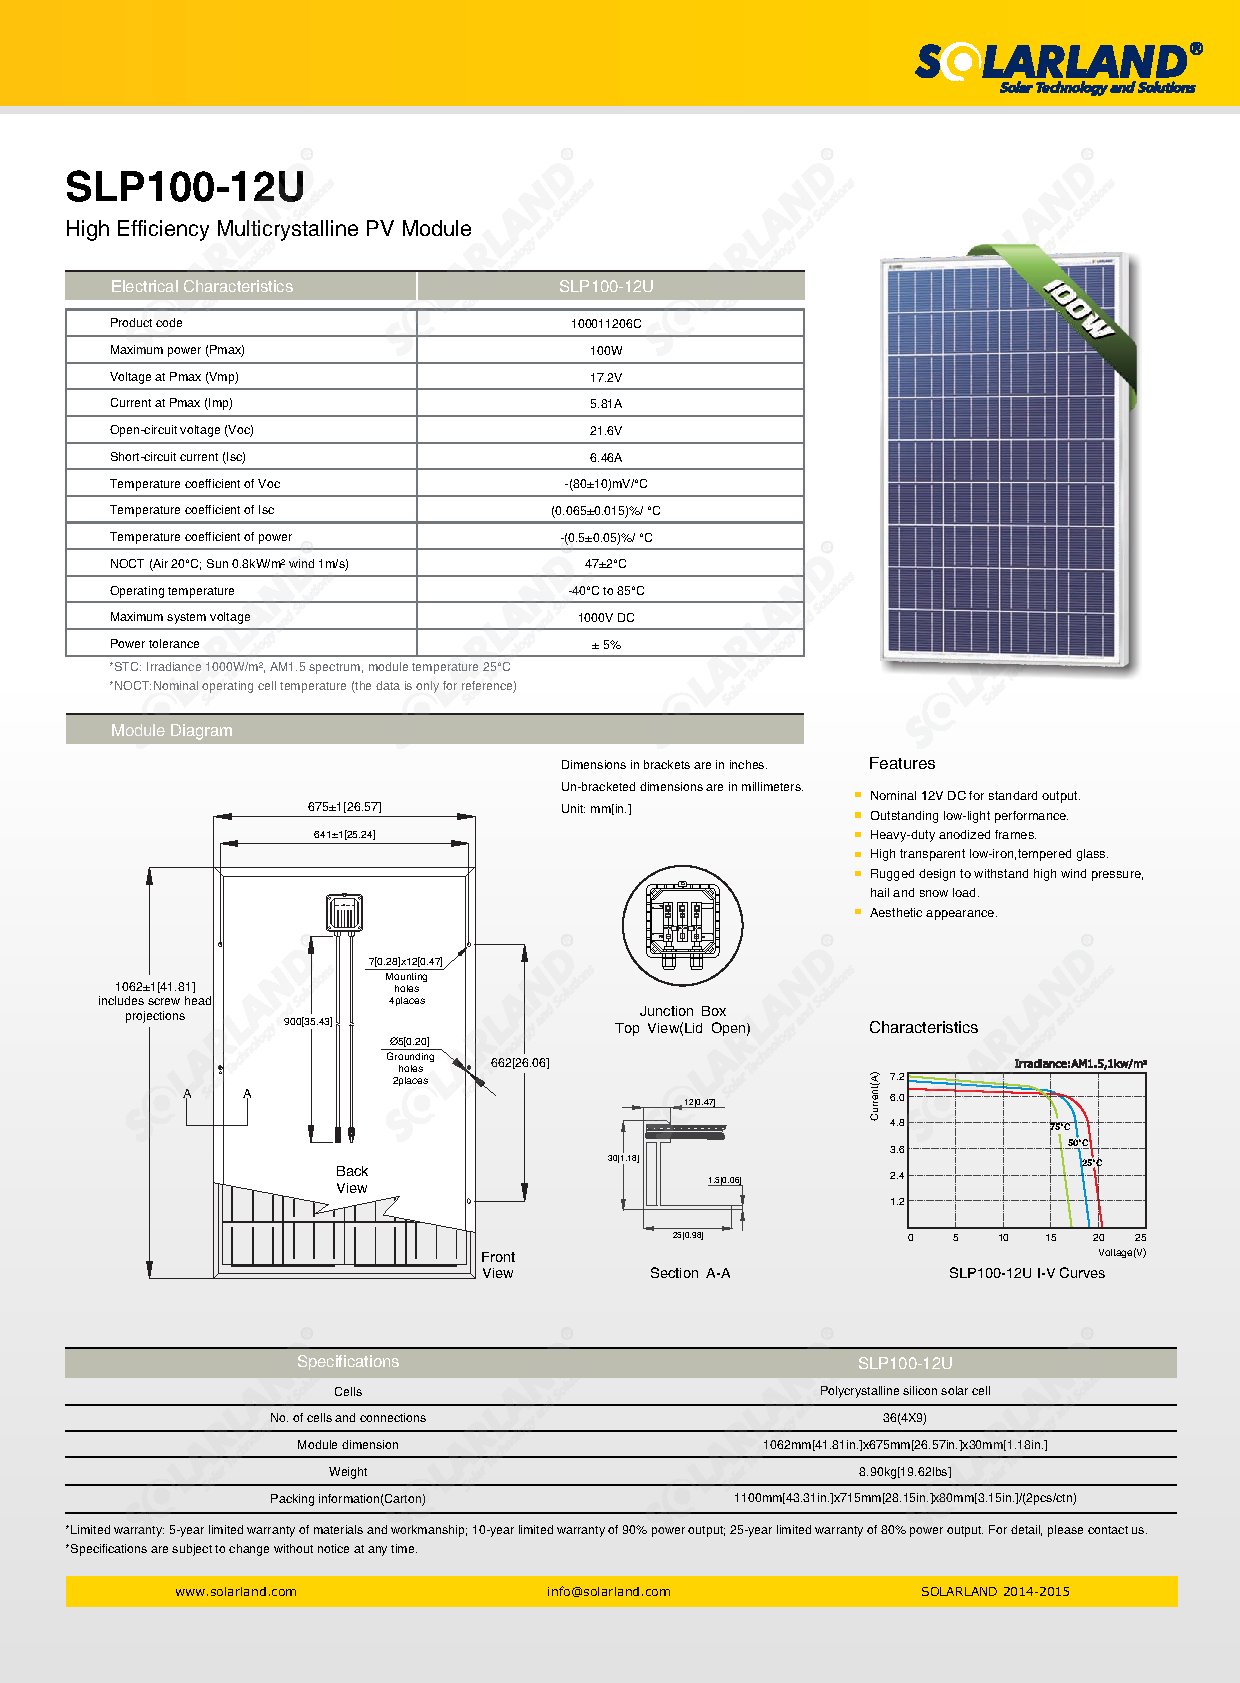
\includepdf[pages=-]{Rigid_Solar.pdf}

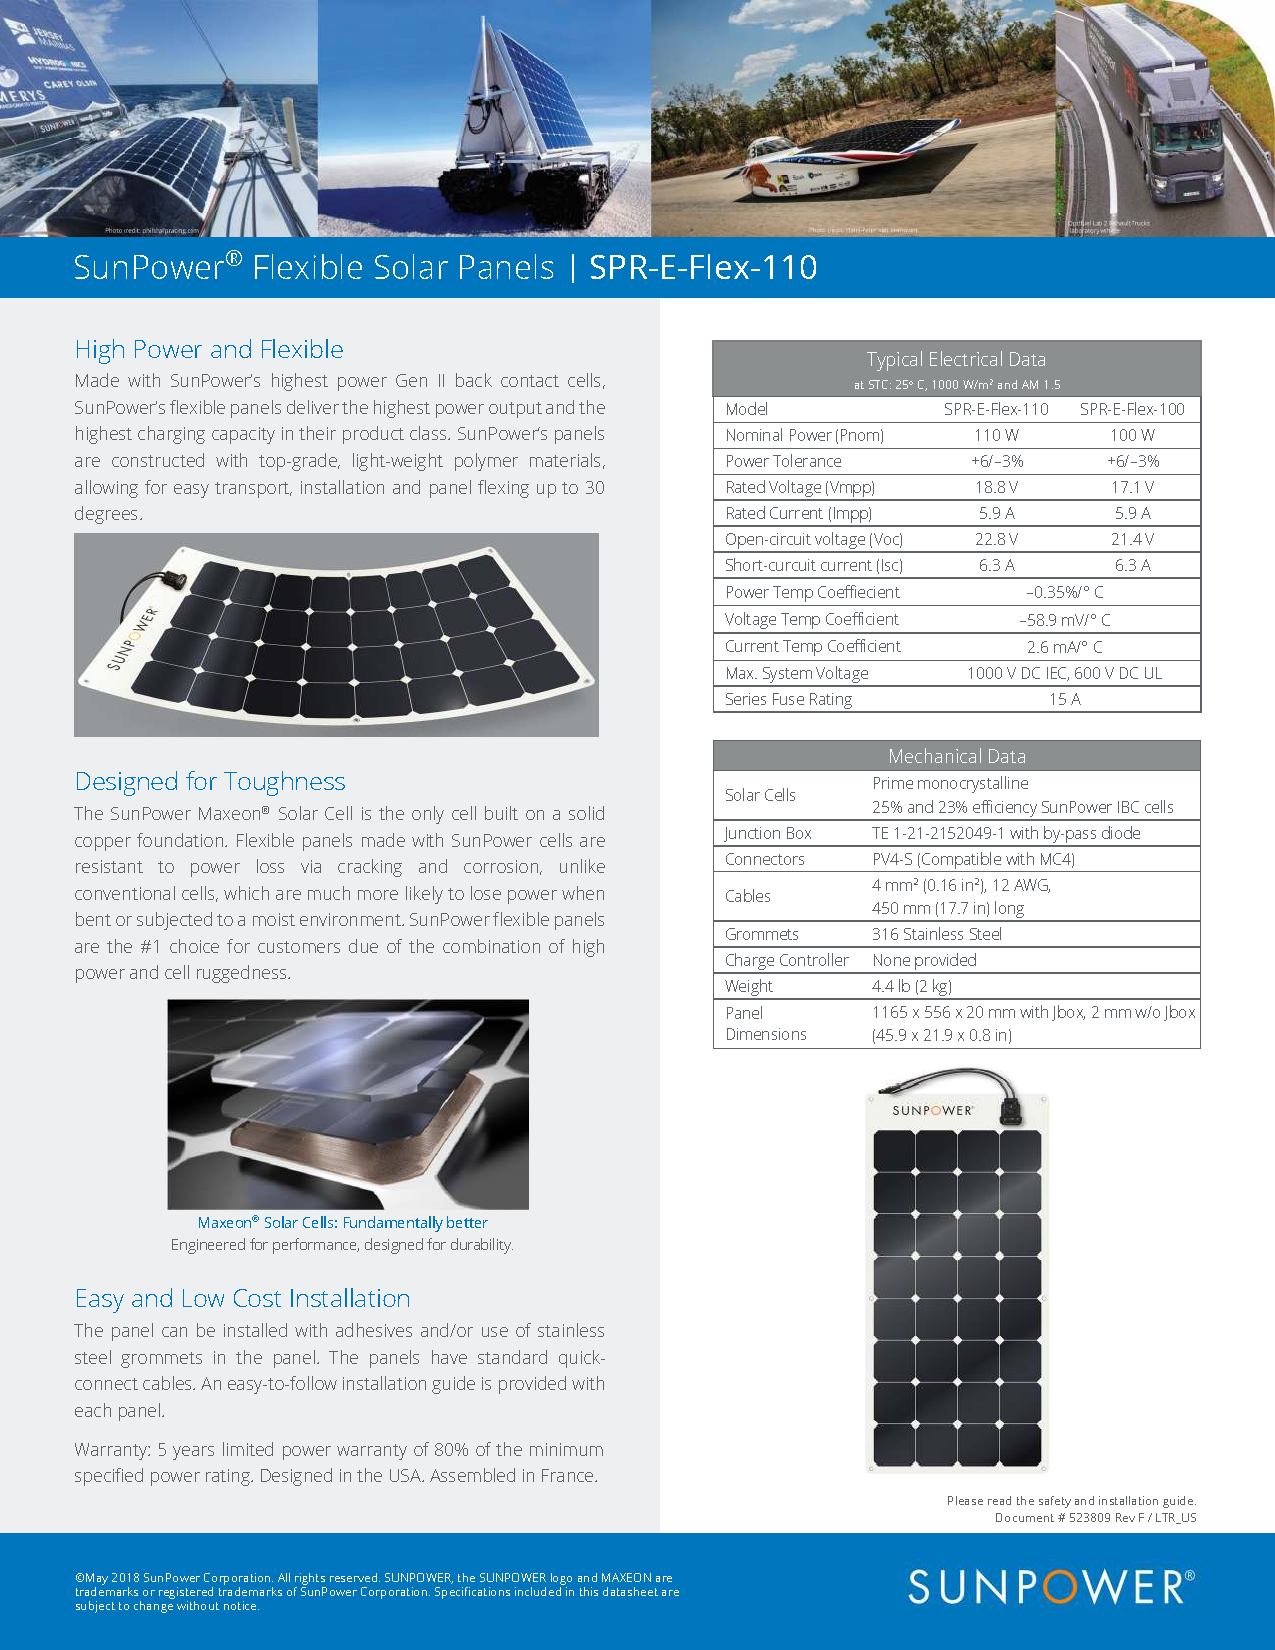
\includepdf[pages=-]{Flex_Solar.pdf}

\subsection{Solar Cells by Sunpower \cite{sunpower_buy_2017}}

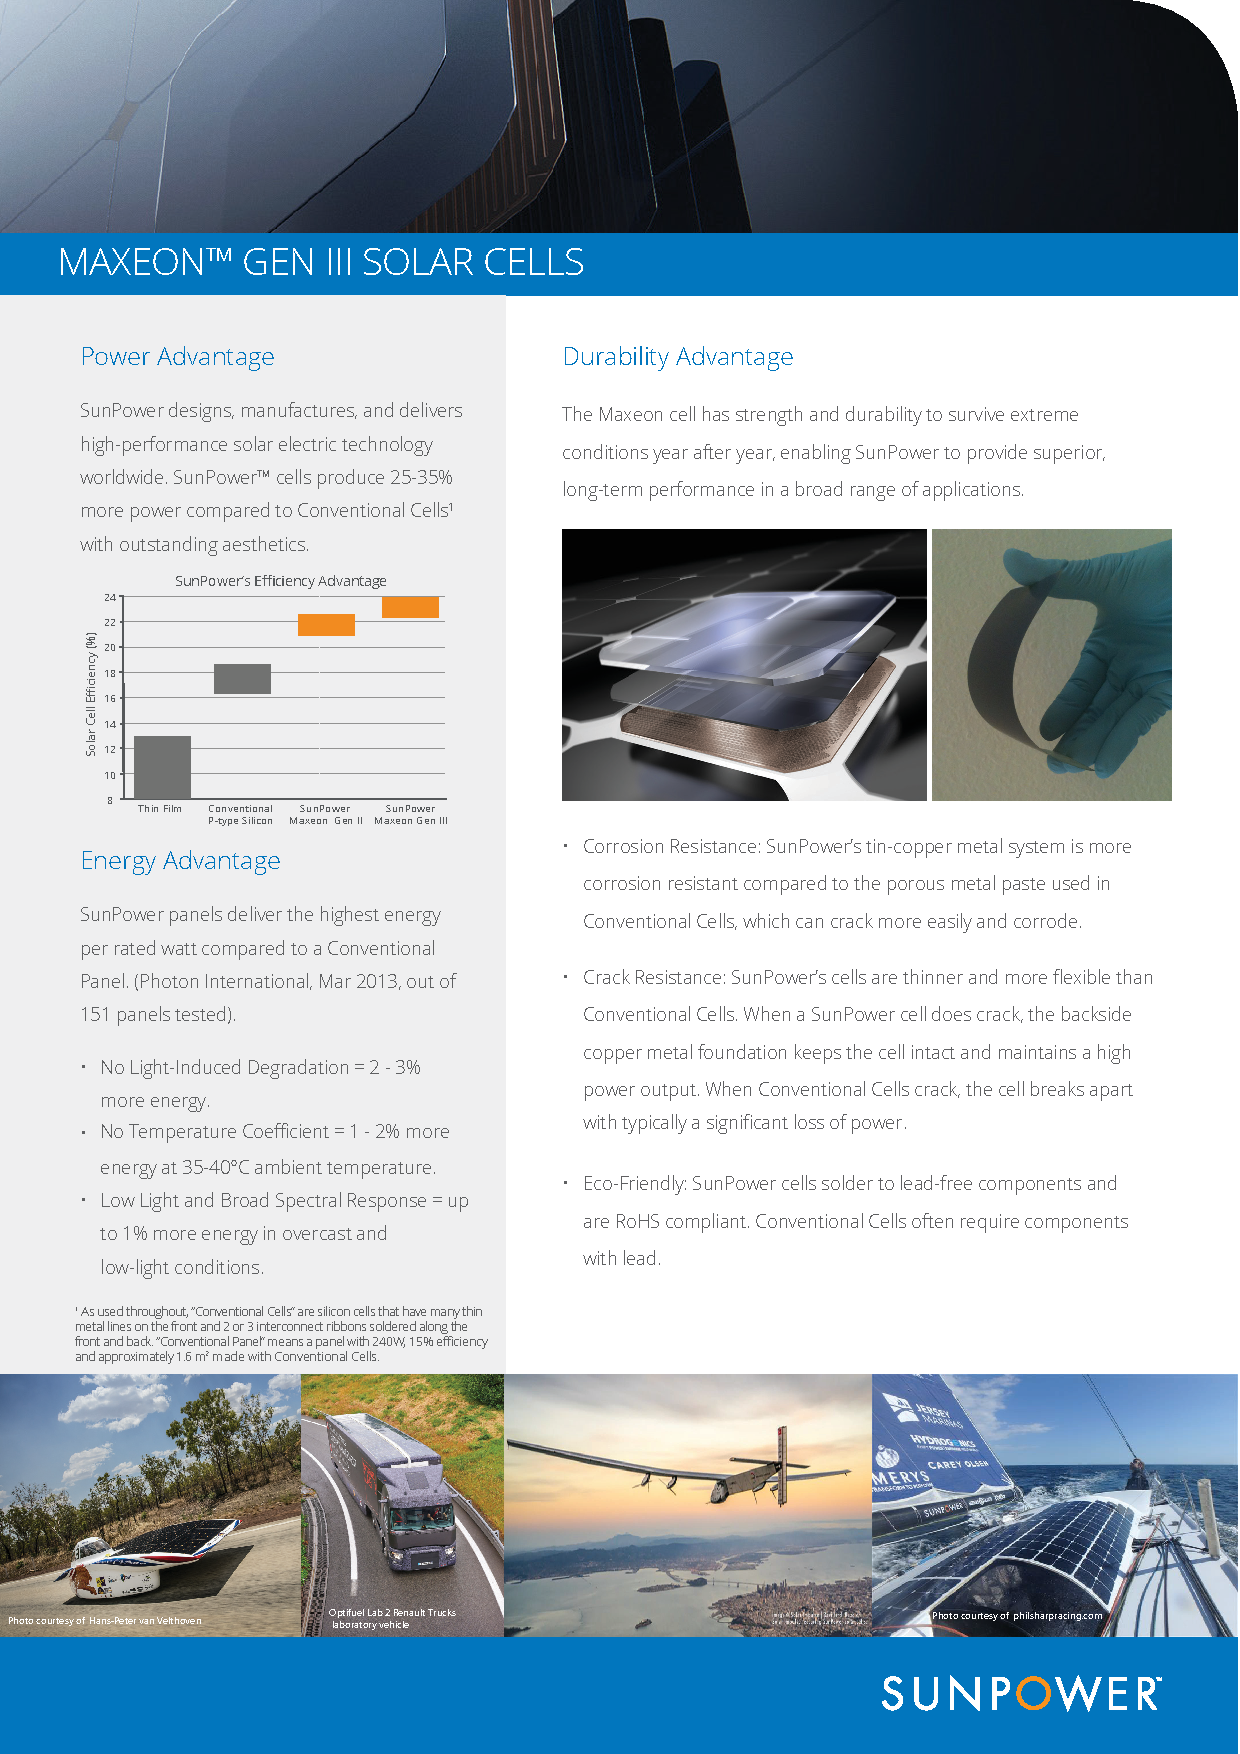
\includepdf[pages=-]{Cell_Solar.pdf}

\subsection{Solar Regulator Specifications from REDARC Electronics \cite{redarc_electronics_20a_nodate}}

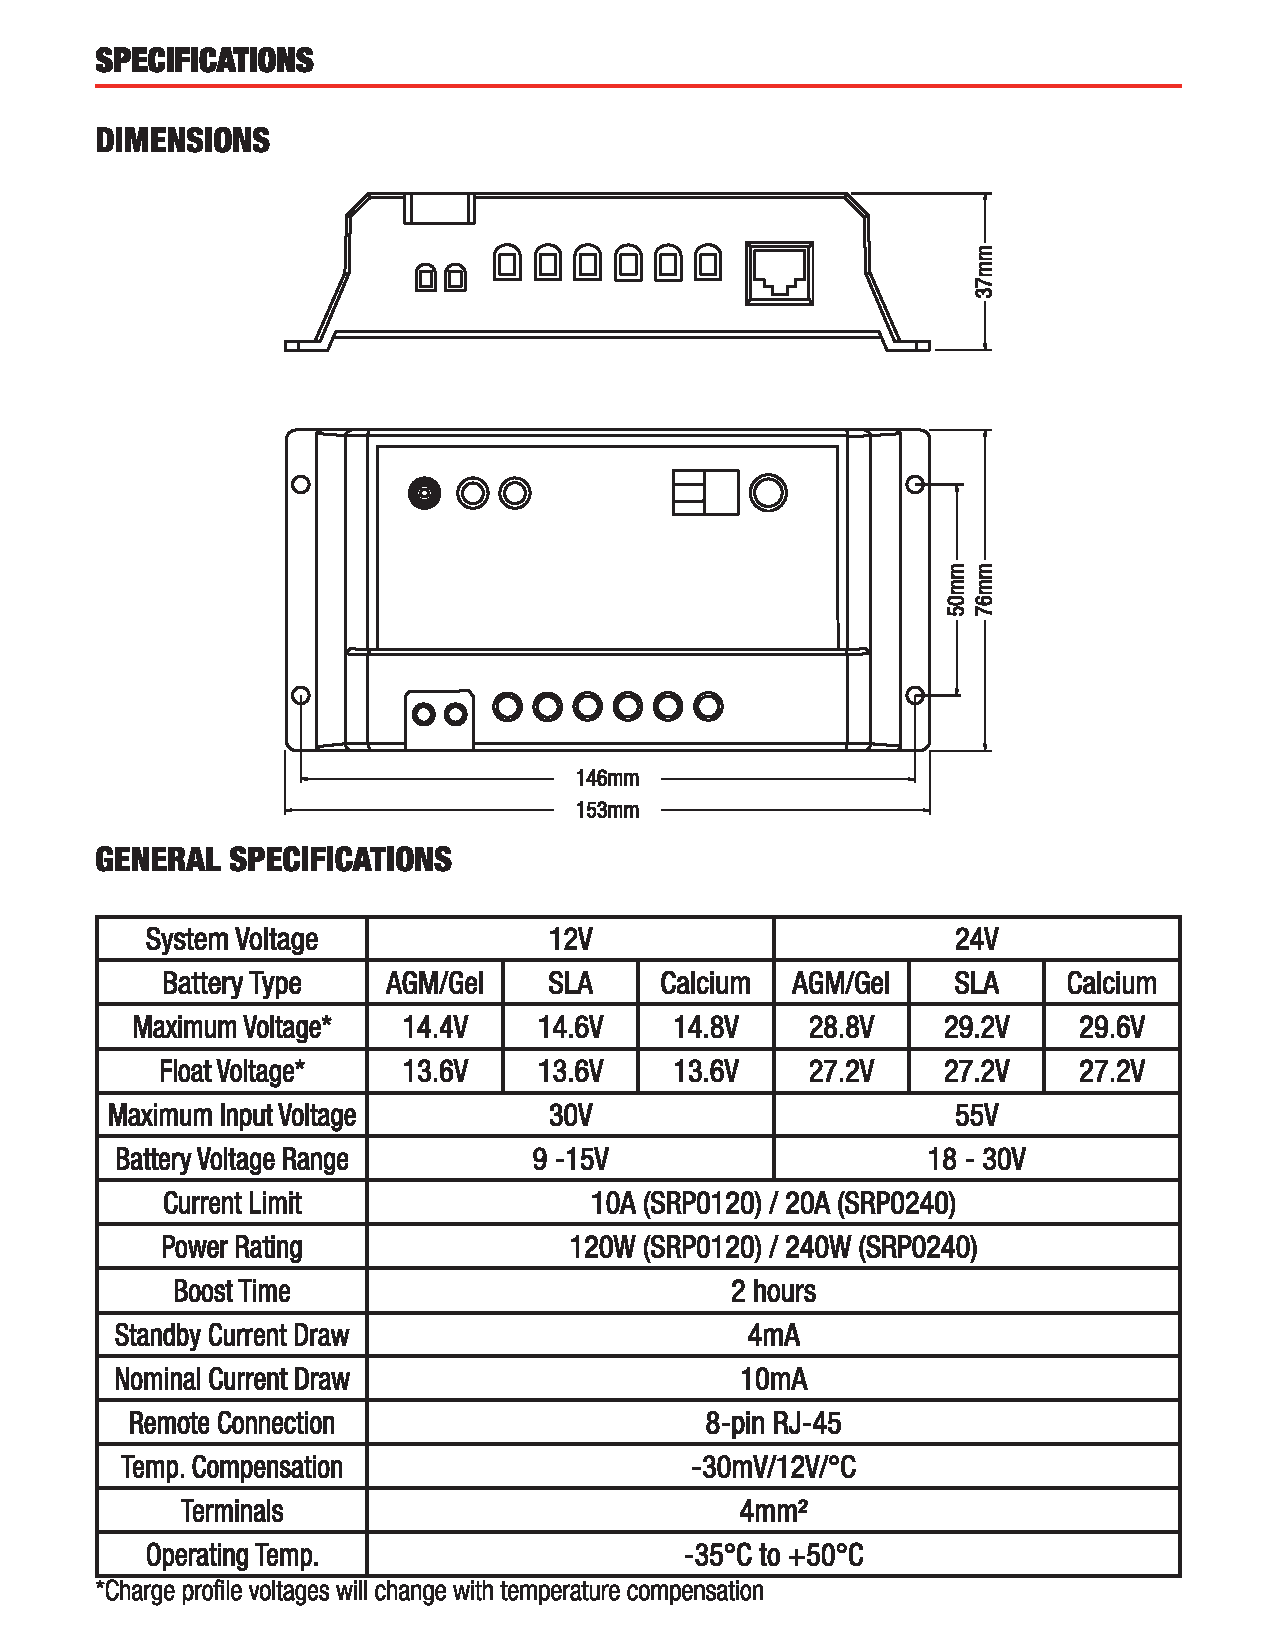
\includepdf[pages=-]{Reg_Solar.pdf}

%------------------------- COOLING -------------------------%

\subsection{Cooling} \label{app:cooling}

\subsubsection{Computer Cooling}

The primary cooling concern of computer cooling is the CPU, which accounts for nearly 50\% of server power consumption; other elements such as memory, hard drives and voltage regulators are cooled passively or take advantage of the CPU cooling solution \cite{kheirabadi_cooling_2016}.

Air cooling is the most well established method of cooling major server components; heat sinks are attached to high flux devices while forced air convection generated by fans pulls heat away from components.
They are generally mounted the same way as PC indirect liquid cooling systems as shown in figure \ref{fig:cooling_cpu_water_experimental}.

\begin{figure}[H]
    \centering
    \includegraphics[width=0.6\textwidth]{Sections/LiteratureReview/img/cooling/std_cpu_air.png}
    \caption{Server air cooling configuration \cite{kheirabadi_cooling_2016}. CRAC = computer room air conditioning; this unit pushes hot air outside and feeds in fresh air}
    \label{fig:cooling_cpu_air}
\end{figure}

Indirect liquid cooling interfaces a coolant liquid to the CPU heat-sink directly before feeding the heat outside.
They allow for decreases power consumption for equivalent cooling, at the cost of higher more infrastructure to avoid leakage and proper piping.

\begin{figure}[H]
    \centering
    \includegraphics[width=0.6\textwidth]{Sections/LiteratureReview/img/cooling/std_cpu_water.png}
    \caption{Server indirect water cooling configuration \cite{kheirabadi_cooling_2016}. CDU = coolant distribution unit}
    \label{fig:cooling_cpu_water}
\end{figure}

An indirect liquid cooling heat-sink for CPUs was developed by Kheirabadi and is shown below \cite{cherom_kheirabadi_experimental_2017}.

\begin{figure}[H]
    \centering
    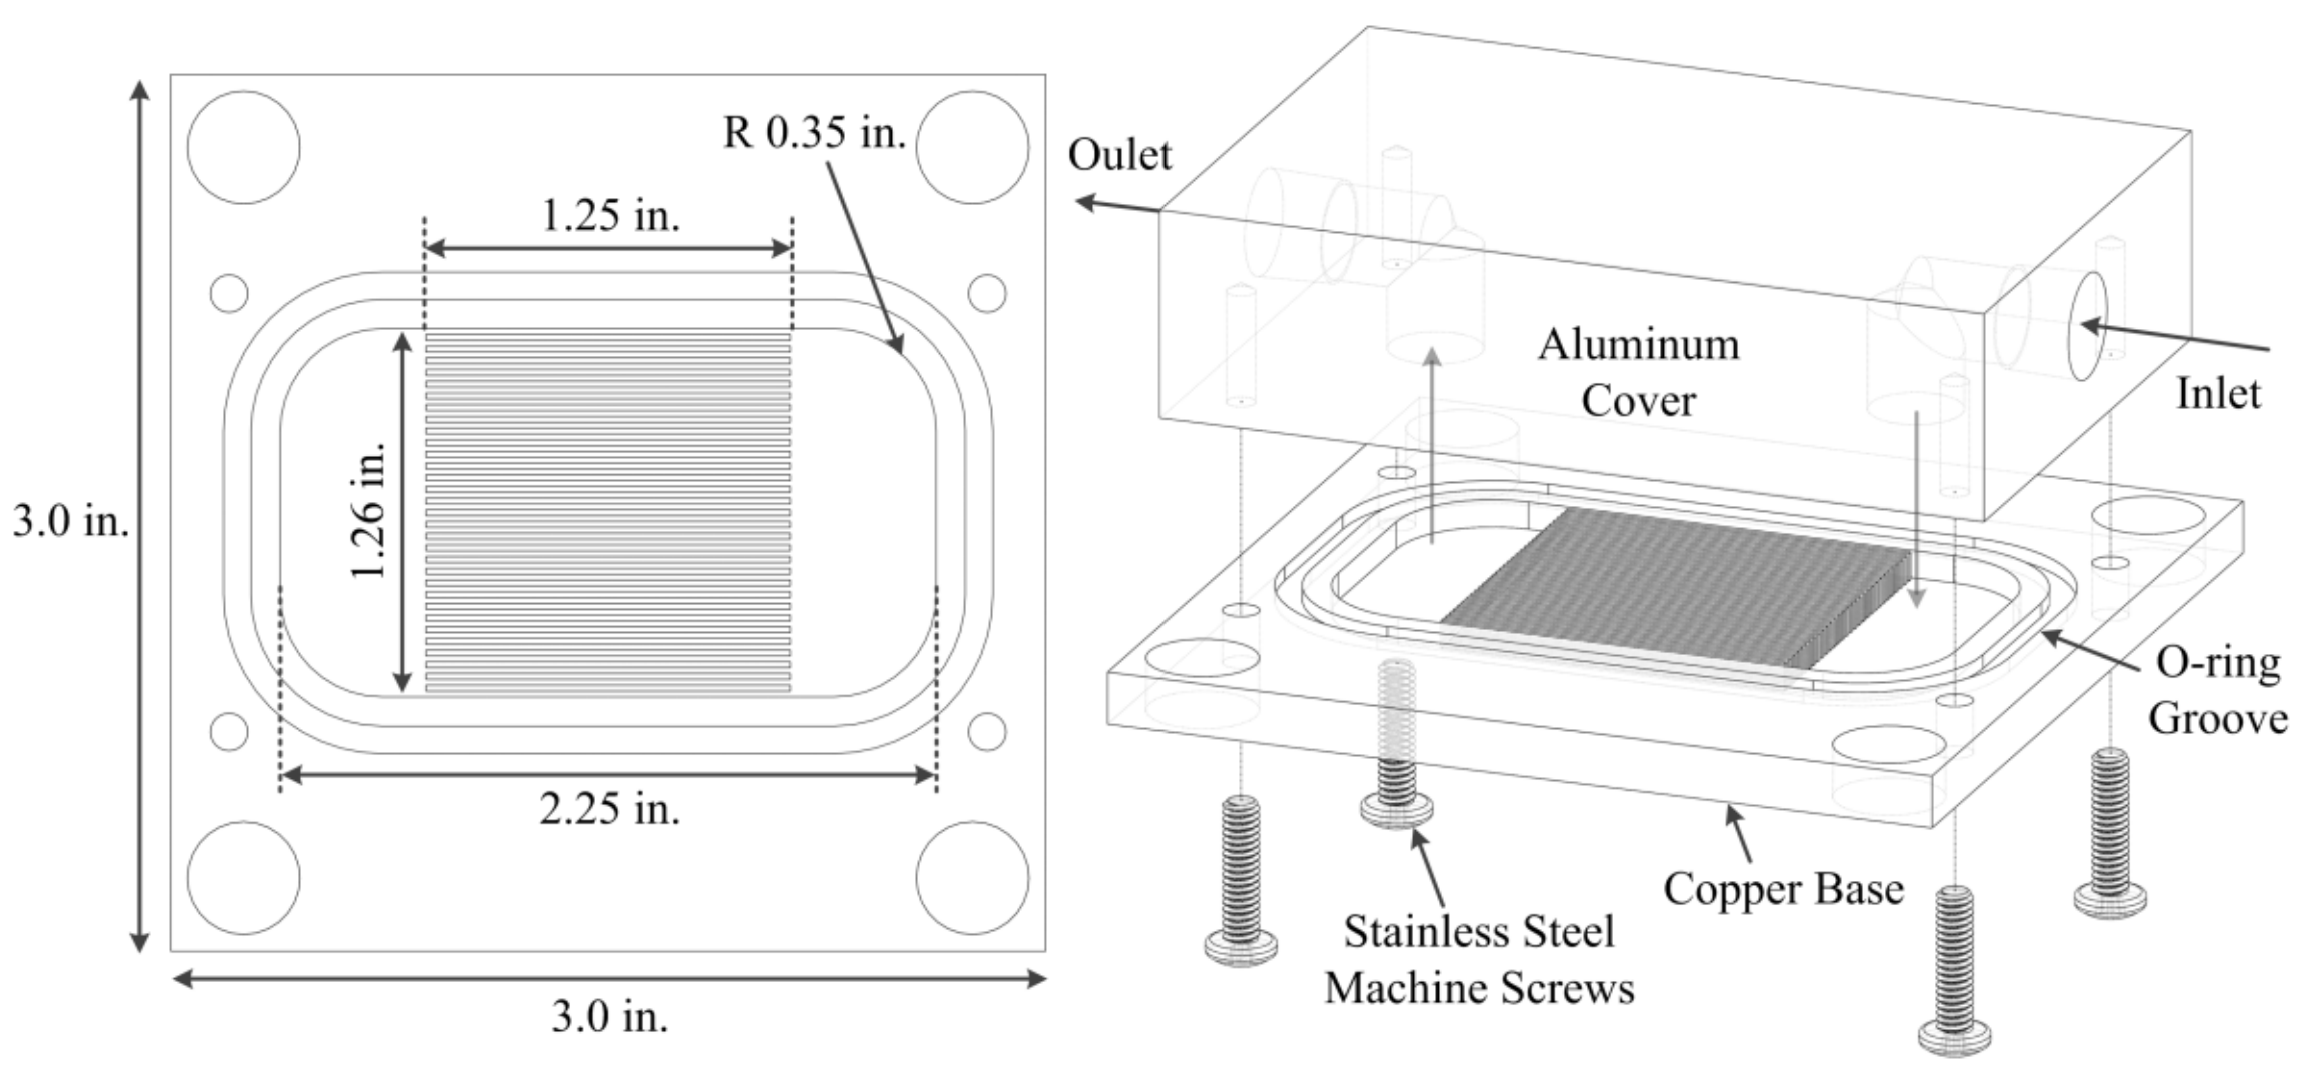
\includegraphics[width=\textwidth]{Sections/LiteratureReview/img/cooling/std_cpu_water_schematics.png}
    \caption{Heat-sink design by Kheirabadi \cite{cherom_kheirabadi_experimental_2017}}
    \label{fig:cooling_cpu_water_experimental}
\end{figure}

The corresponding heat exchanger plate is shown below (equivalent to the chiller element from figure \ref{fig:cooling_cpu_water}).

\begin{figure}[H]
    \centering
    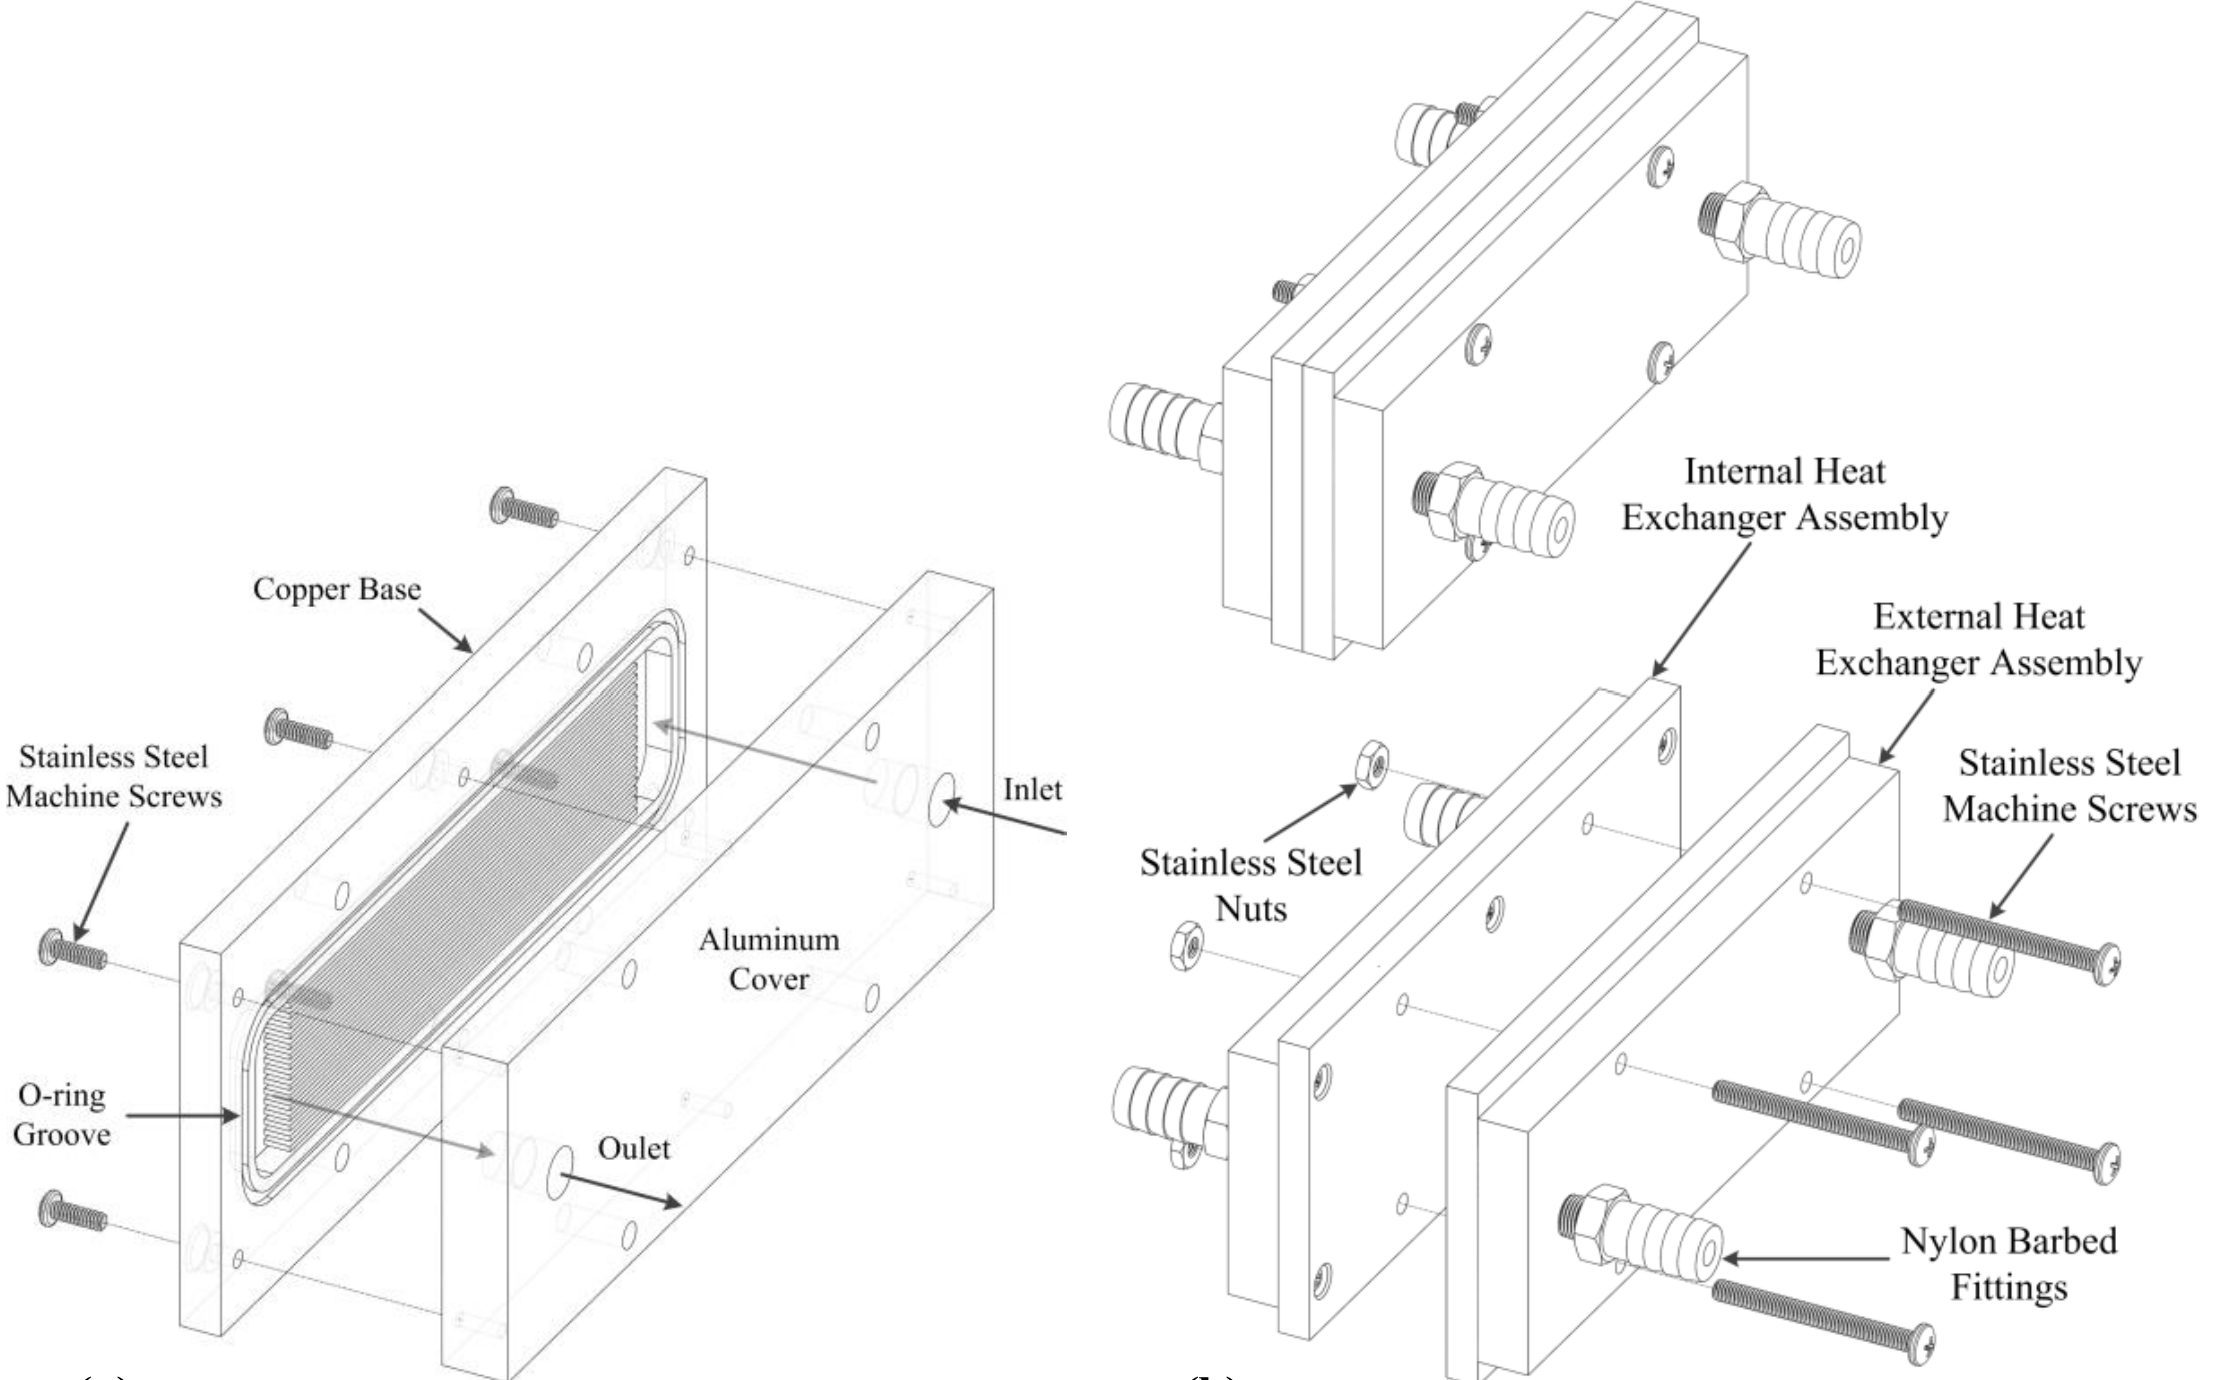
\includegraphics[width=0.8\textwidth]{Sections/LiteratureReview/img/cooling/std_cpu_water_exchanger.png}
    \caption{Heat exchanger design by Kheirabadi \cite{cherom_kheirabadi_experimental_2017}}
    \label{fig:cooling_cpu_water_experimental_exchanger}
\end{figure}

Other solutions such as pool boiling and direct liquid cooling exist, however these are more esoteric.

\subsubsection{Actuator Cooling}

Traditionally, actuators are cooled by forcing air through their housing using an external blower motor and fan, as shown in figure below \cite{noauthor_chapter_nodate}.

\begin{figure}[H]
    \centering
    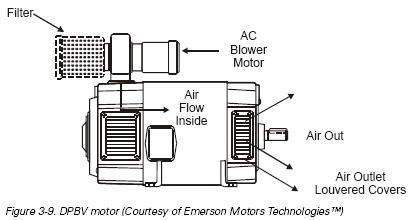
\includegraphics[width=0.9\textwidth]{Sections/LiteratureReview/img/cooling/std_motor_cooling.png}
    \caption{Traditional DC motor cooling technique \cite{noauthor_chapter_nodate}}
    \label{fig:cooling_motor_standard}
\end{figure}

Boats with inboard motors (where the motor is not exposed to the outside) use a system of liquid coolant (typically antifreeze) to direct heat away from the motor, and exchange heat with seawater.

\begin{figure}[H]
    \centering
    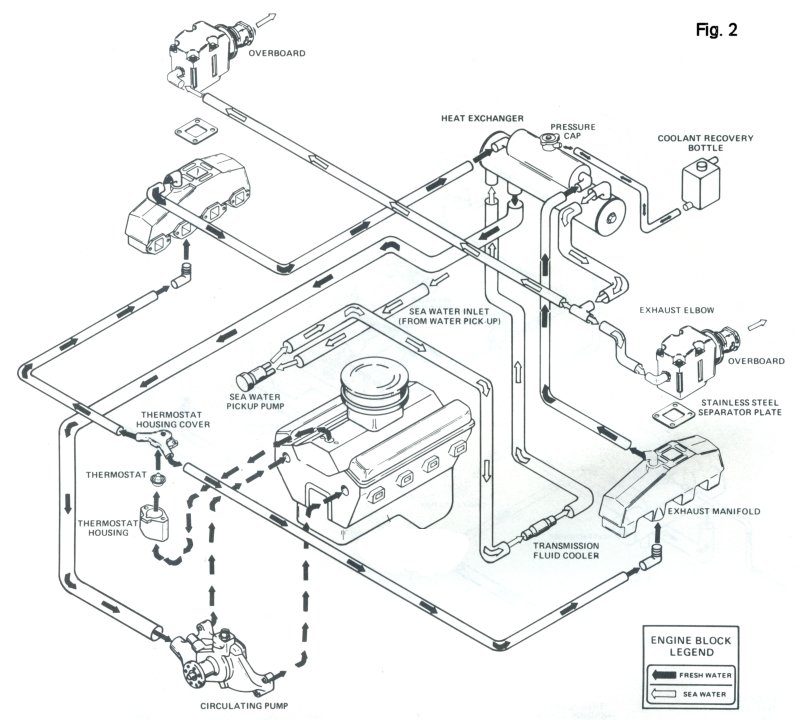
\includegraphics[width=0.9\textwidth]{Sections/LiteratureReview/img/cooling/std_motor_cooling_boat.jpg}
    \caption{Boat inboard motor cooling system \cite{noauthor_inboard_nodate}}
    \label{fig:cooling_motor_boat_inboard}
\end{figure}




%-------- Motor Specs
\subsection{Motor and Component Specifications} \label{app:motor_comp_spec}

\subsubsection{Specification for the Brushless DC Motor 24V 4000RPM \cite{robots_shop_24v_nodate}}
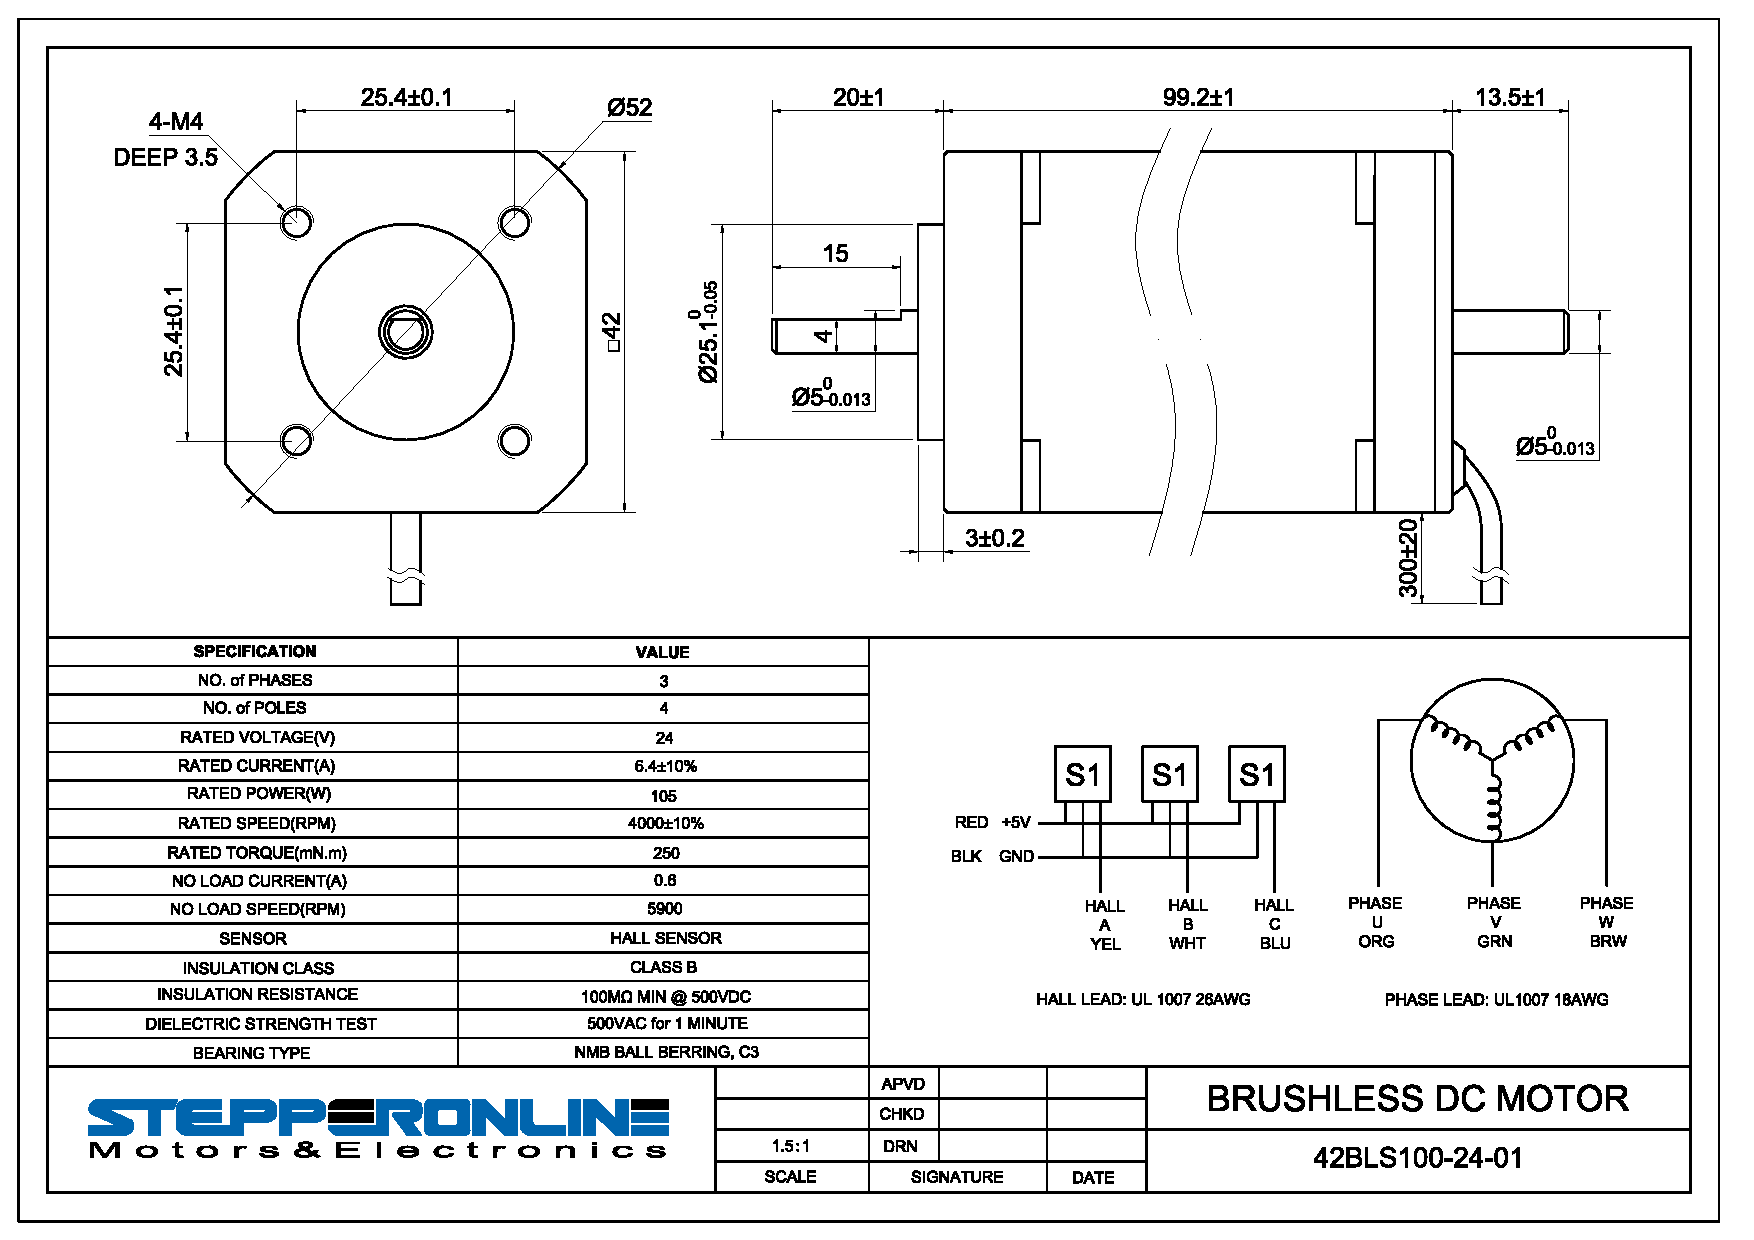
\includepdf[pages=-]{DC_Motor_Specs.pdf}

\subsubsection{Specification sheet for the planetary gear \cite{banggood_nema_nodate}}

\begin{figure}[H]
    \centering
    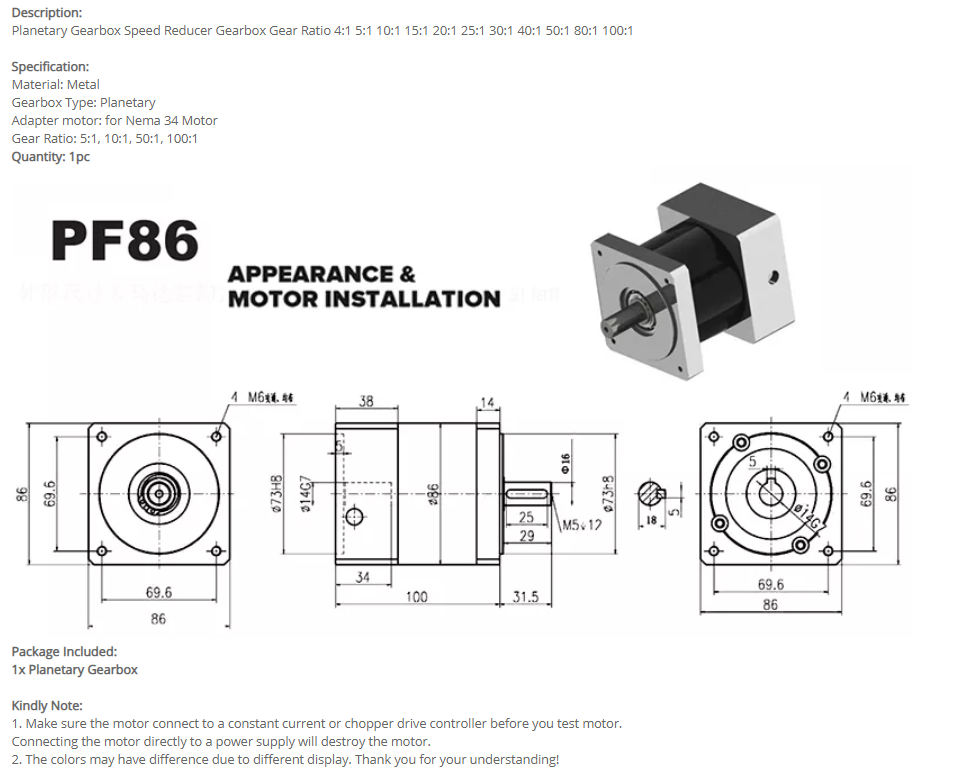
\includegraphics[width=0.98\textwidth]{Sections/Appendices/GearBox_specs.PNG}
    \caption{Gearbox Specifications \cite{banggood_nema_nodate}}
    \label{fig:gearbox_spec}
\end{figure}

\subsubsection{Specification sheet for the DC gearmotor \cite{mcmaster-carr_gearmotors_nodate}}
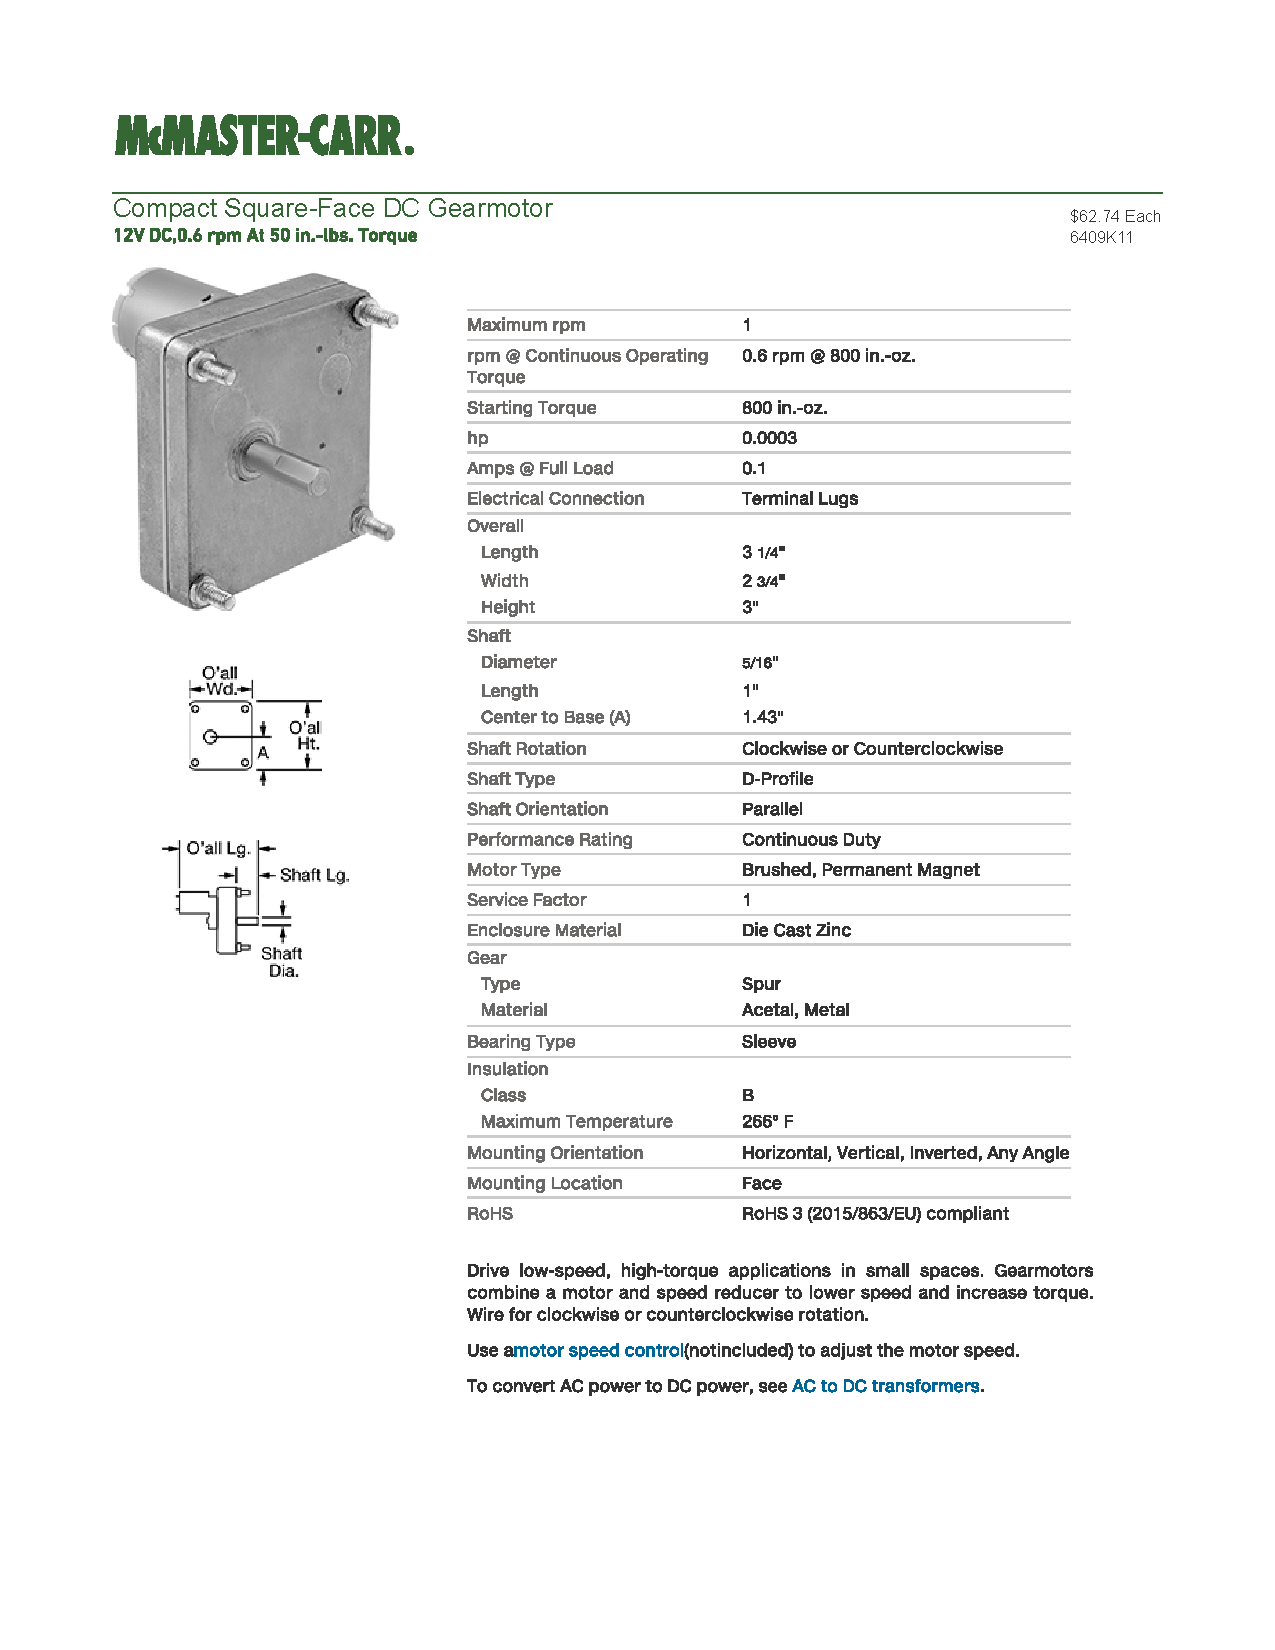
\includepdf[pages=-]{McMaster-Carr.pdf}


\subsubsection{Specification sheet for the gearmotor \cite{acklands_grainger_dc_nodate}}
\begin{figure}[H]
    \centering
    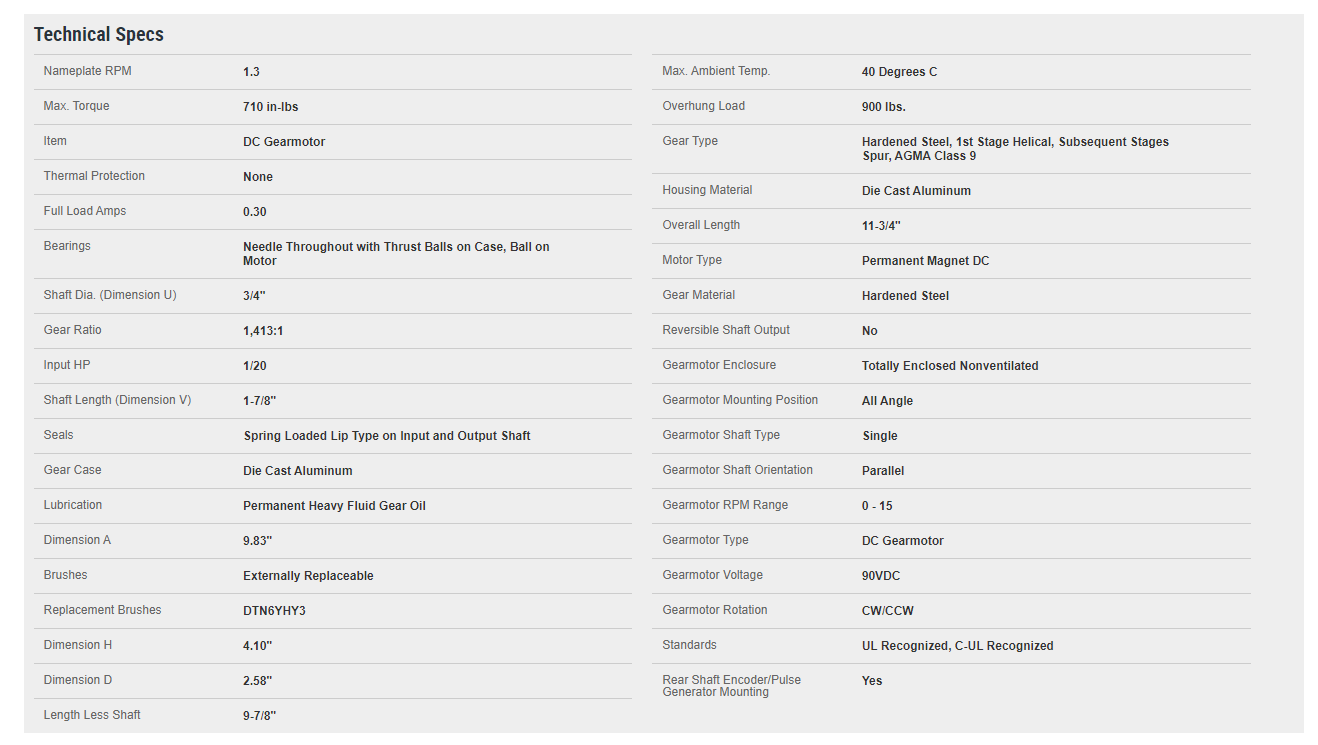
\includegraphics[width=0.98\textwidth]{Sections/Appendices/SpecsAcklandMotors.PNG}
    \caption{Acklands Grainger 90VDC Gearmotor Specifications Sheet \cite{acklands_grainger_dc_nodate}}
    \label{fig:ackland_spec}
\end{figure}
